%!TEX root = ../thesis.tex

\chapter{Approach}
\label{ch:approach}

\section{Introduction}
 In chapter 2 we discuss the object of the thesis, which is to design and develop the workflow that enables organizations to share their datasets for consumption by users from other organizations without exposing the dataset itself. And the system that we are trying to develop should allow users to write code without developing expertise to write distributed code like Hadoop's MapReduce Jobs.
 
 \bigskip
 This thesis is part of a bigger proof of concept that incorporates this system together with Distributed Identity Framework (DID) and authenticator for JupyterHub as well as integrating this with the NFT Framework for proving ownership and stake in data as well as results. The integration between the workflow and other parts of the final proof of concept does not fall under the scope of this thesis.
 
 \bigskip
 The overview of our approach is briefly demonstrated in \ref{fig:component-jobs}. We set up a Hyperledger network using docker-compose with three organizations and smart contracts/chaincode that will be invoked by a REST API. The REST API is an application that will be owned by the organization and can be made internal to the organization since it will be interacting and storing with the MySQL database to store keys for encryption/decryption of sensitive data before committing to the blockchain. However, as part of this proof of concept, we only create one instance of the API. As the next step, we set up a Kubernetes cluster and install Argo and JupyterHub on the cluster. The users can log in to this JupyterHub environment to use it as an IDE and explore the datasets available. We develop a custom extension for JupyterHub for navigating the datasets and develop JupyterFlow further to create Persistent Volumes, mount Persistent Volume Claims on Kubernetes, and create Argo Workflow from a template and trigger the workflow with those volumes mounted for jobs requiring the data.

\bigskip
Before delving into the details of the implementation we want to acknowledge that the work we present here is only a proof of concept and contains several loopholes and security vulnerabilities that need to be addressed in future work before this work can be considered to be production-ready. Moreover, we assume that one organization takes charge of initiating the consortium and that organizations agree to the policies and rules before joining in. Moreover, we acknowledge the system can be exploited very easily given that the secrets after reading from the blockchain are stored in a plain text hidden file and are only secure by obscurity. This can be improved later to stop the user from reading these sensitive values. Moreover, the details like user id and roles will be available from the Distributed Identity framework once integrated, which right now are input and any user can take the role of any other user.

\section{Proposed Solution \& How it Works}

\begin{figure}
    \centering
    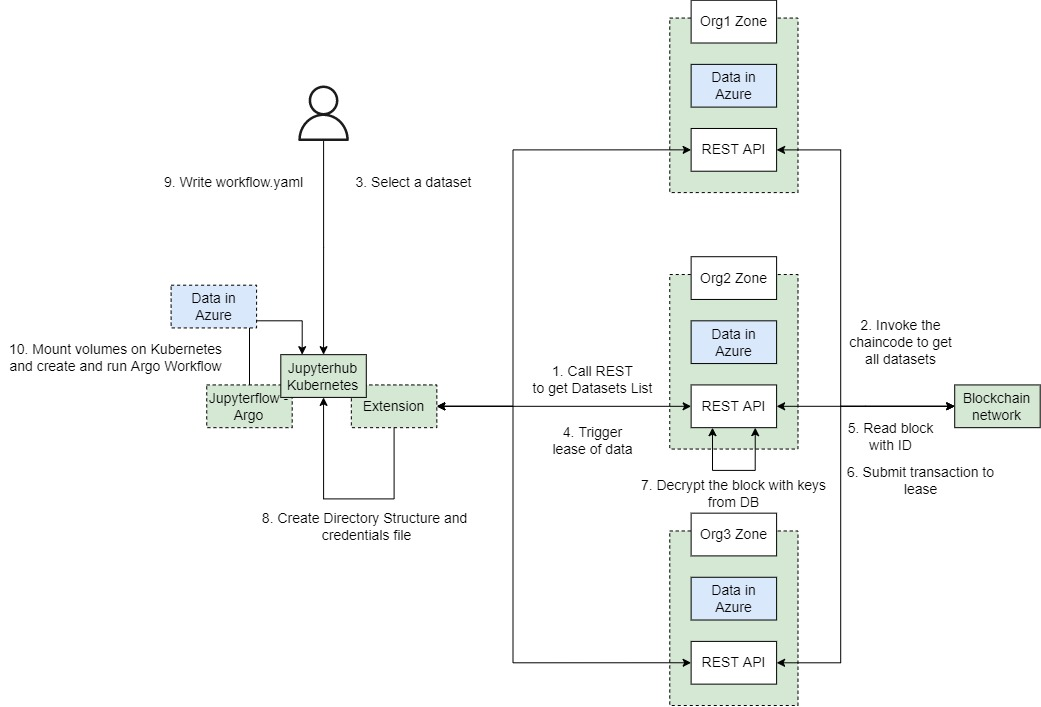
\includegraphics[width=14cm,keepaspectratio]{photos/how-it-works-2.jpg}
    \caption{Step by step process of the workflow of the information and instructions in the system.}
    \label{fig:how-it-works}
\end{figure}
Figure \ref{fig:how-it-works} highlights a step-by-step process of how the entire proof of concept works to consume datasets from multiple sources in a workflow without ever sharing the ownership and not allowing the user to even see the data.

\begin{enumerate}
    \item Read a list of all the datasets available from the Hyperledger Fabric network by calling the REST API that invokes the necessary chaincode.
    \item User selects one or more datasets to consume in jobs inside the workflow that will be triggered later.
    \item The extension triggers the lease endpoint in the REST API.
    \item The REST API invokes the chaincode that will submit the transaction to lease the data. If the data is free it will be leased else an error thrown.
    \item The chaincode to get the block using the ID is invoked. The REST API gets the decryption keys for the specific data block from the database and returns the decrypted data.
    \item Extension received a response from the API and creates a directory structure for the user to experiment with and write the code.
    \item Extension creates a hidden file with the credentials to mount the data as a persistent volume claim in Kubernetes.
    \item User writes a \lstinline{workflow.yaml}
    \item JupyterFlow creates a persistent volume on Kubernetes, creates a claim, and uses those claims for relevant jobs. Creates an Argo Workflow and triggers it.
    \item The Argo workflow runs and computes the results.
\end{enumerate}

\section{Implementation Details}
\subsection{Setting up Blockchain Network}
In the system we propose organizations will be storing metadata about their datasets on a blockchain to have full control of themselves and not a trusted third party that in traditional architecture will be maintaining the system. We will set up a blockchain network in Hyperledger Fabric with three organizations and one orderer organization. Each organization in the test network will contribute only a single peer node.

\bigskip
Since Hyperledger is a permissioned/private blockchain, every entity on the chain needs private keys and certificates following public key infrastructure issued by a certified authority to identify them. In a production scenario, each organization will have a different CA who will be responsible for providing certificates not only for the users but also for the peer nodes. In our test environment, we use the CA tools provided by Hyperledger designed and available specifically for test environments. We spin up docker containers for each organization and the identities of an admin, a user, and a peer are generated by the CA. We enroll them in the respective organizations as part of the setup process.

\bigskip
Hyperledger uses the identities to identify the participating entity and see if the policies allow the specific entity to perform the requested operation. Policies are rules that each organization sets up when joining a channel to specify who can perform which operations on the network. Consider the following policies that we have for UiS (One of our test organizations). For testing, we use the same policies for each organization. These policies can be configured in \lstinline{configtx.yaml} and each organization can write its own users' and peers' policies according to its internal structure.

\begin{lstlisting}[caption={Policies for UiS (one of our test organization). We use the same policies for other organizations as well.}]
Policies:
    Readers:
        Type: Signature
        Rule: "OR('UiSMSP.admin', 'UiSMSP.peer', 'UiSMSP.client')"
    Writers:
        Type: Signature
        Rule: "OR('UiSMSP.admin', 'UiSMSP.client')"
    Admins:
        Type: Signature
        Rule: "OR('UiSMSP.admin')"
    Endorsement:
        Type: Signature
        Rule: "OR('UiSMSP.peer')"
\end{lstlisting}

\bigskip
So we have four roles stating who can read, write, administer the organization (Add users, peers, etc.) and endorse transactions. And policies can use AND, OR and other binary operators to define rules for each role. Here we want to highlight also why participants need to be enrolled in the MSP because the network uses MSP to attach identities to their roles. As an example, once an entity is registered in the MSP either as an admin, peer (because chaincode runs with peers identity), or a user they are eligible to read from the ledger.

\bigskip
We have already seen the policies that dictate in a network and that they are specified in a \lstinline{configtx.yaml} file. \lstinline{configtx.yaml} hosts a few other configurations as well in addition to the policies. In this file, first, we define the organizations in the network with the name, location for identities, and policies for each organization. Also, keep in mind that organizations can later be added to the network. That is the reason we set up a network with two test organizations and add a third one later but we will discuss more on that in \ref{ch:eval}. Next, we configure the capabilities section which is left default since this section is internal to Hyperledger to dictate which features are available in the version being used. The application-level configuration and policies dictate how smart contracts are configured to behave and which organizations are allowed to endorse the addition of a new version of a chaincode or a new chaincode altogether on the channel. And finally, we have the profile configuration, stating the organizations that will be part of an application channel.

\bigskip
After the initial setup, we create similar configurations for the third organization and follow the same procedure to add it to the channel by creating identities and enrolling these identities with the MSP, and then adding them to the channel we created previously. The only difference is that the Majority of other organizations need to approve or endorse when adding a new organization as specified in the policies of the application channel when setting up the network.

\subsection{Chaincode}
Hyperledger applications can not read or update the ledger directly, rather they interface with the blockchain and the ledger through the chaincode. Chaincode is Hyperledger terminology for smart contracts and contains the business logic of the network whenever processing a transaction on the block. So chaincode is a vital part of any network.

\bigskip
As mentioned before, Hyperledger, unlike other blockchain frameworks provide the opportunity to write chaincode in languages like Go, Java, and NodeJS. We develop our chaincode in JavaScript. Chaincode needs to implement the Contract class provided by the fabric-contract-api package for Node. And each method in the class is auto-injected with context that allows it to read from the world state of the ledger and submit transactions to modify the ledger. The transactions then need to be endorsed by peers from other organizations as stated in the policies when setting up the channel. These methods are then invoked by external, off-chain applications in our case the REST API.

\bigskip
Each block on the chain is metadata about a dataset that an organization wants to share. And apart from the organization having complete control over who can access this on the blockchain, this being a ledger we are continuously getting an immutable log of who and when updated the block and also who the dataset was leased to. As part of designing the workflow that allows for the consumption of data, a Create, Read, Update and Delete (CRUD) chaincode would suffice. In addition to the update chaincode, we have another chaincode that only leases a dataset from one organization to another after validating that the dataset is not in use. 

\bigskip
Here are the outlined steps needed to add chaincode to the channel and are implemented in \lstinline{deploy.sh}. Also mentioned are the commands for each step.

\begin{itemize}
    \item \textbf{Packaging} The first step is to package the chaincode into a tar archive. If same chaincode is going to be running for every organization then only one organization can complete this step and share the packaged code off-channel. 
    \begin{lstlisting}[language=bash]
        peer lifecycle chaincode package data-chaincode.tar.gz --path chaincode/ --lang node --label data-chaincode-1\end{lstlisting}

    \item \textbf{Installation} Each organization intending to use the chaincode needs to install the chaincode on their peers.
    \begin{lstlisting}[language=bash]
    peer lifecycle chaincode install data-chaincode.tar.gz\end{lstlisting}
    
    \item \textbf{Approval} Organizations need to approve a chaincode before it can be added to the channel. \lstinline{LifecycleEndorsement} in \lstinline{configtx.yaml} dictates how many organizations need to approve a chaincode before it is considered eligible to be added to the channel. By default and in our scenario this policy is set to Majority so a chaincode has to be approved by a majority of organizations before it will be installed on the peers.
    \begin{lstlisting}[language=bash]
    peer lifecycle chaincode approveformyorg -o --ordererTLSHostnameOverride --channelID --name  --version 1.0 --package-id --sequence --tls --cafile\end{lstlisting}
    
    To this command we provide orderer address, channel id, chaincode name and version, package id gotten from 
    \begin{lstlisting}[language=bash]
    peer lifecycle chaincode queryinstalled \end{lstlisting}
    
    And the certificate for the approving organization. Moreover, this command picks the MSPID, and peer address from environment variables.
    
    \item \textbf{Commit} Once the chaincode has garnered the required number of approvals, the chaincode can be committed to the channel. Once it has been approved only a single organization can do this step and submit the transaction for the commit of the chaincode definition.
    \begin{lstlisting}[language=bash]
    peer lifecycle chaincode commit\end{lstlisting}
    
    Similar to the last command we provide the path to certs and orderer address.
\end{itemize}

\bigskip
Once the chaincode has been committed, it is now ready to be invoked by applications hosted off-channel. Hyperledger provides several SDKs to develop applications that have the capability to connect to the network through a gateway and invoke the chaincode. The SDK is available in Go, Java, NodeJS, and the SDK for Python is in development. We will be using the NodeJS SDK in our REST API that will be invoking the chaincode.

\subsection{REST API}
To enable communication between the extension developed for JupyterHub and the blockchain network in Hyperledger we set up a REST API. The REST API also can store and retrieve the encryption/decryption keys in a MySQL database. This REST API is the application we were shown in the Hyperledger Sample Network figure \ref{fig:hyperledger-sample-network}.

\bigskip
The Minimum Viable Product (MVP) API that we introduce here should be internal to each organization since this setup also introduces a MySQL database to store encryption keys but in this thesis, for the sake of simplicity, we set up and use one application only. And since transactions to the blockchain can be long-running we also introduce a Redis Cache. We set up MySQL database and Redis as docker containers, the credentials to connect can be set in the environment variables and the NodeJS API can read it from there. MySQL is initialized by running the following queries.

\begin{lstlisting}[language=SQL,caption={Database initialization queries to create user, database and table consumed by the application}]
CREATE DATABASE thesis;

USE thesis;

CREATE USER rest_sa IDENTIFIED BY 'rest_sa_pwd';  

CREATE TABLE key_mappings (
  id varchar(255) not null,
  crypto_key varchar(255) not null,
  iv varchar(255) not null
);

GRANT ALL PRIVILEGES ON thesis.* TO 'rest_sa'@'%';
\end{lstlisting}

\bigskip
As we know in a Hyperledger network, each user needs to be identified when interacting with the chain. How we enable that in an application, is that the application interacting with the blockchain hosts a wallet. A wallet is nothing more than just a collection of user identities. Each application that interacts with Hyperledger can maintain a wallet and at run-time one of these identities is selected and used when connecting to a channel. At the startup of the API, we use the identities generated by the CA and provided to the MSP to create a File System wallet for users. In a production-ready system, the File System wallet should be replaced with a CouchDB wallet. The concept of a wallet for application interfacing with the blockchain can be read up from \footnote{\url{https://hyperledger-fabric.readthedocs.io/en/release-2.2/developapps/wallet.html}}.

\bigskip
After an identity has been selected from a wallet, the application can connect to the channel and invoke chaincodes, and submit transactions. The connection to the channel is initiated and maintained by creating a gateway to the network, which is created using configurations specified in a connection profile. A connection profile is generated when an organization is added to the blockchain network. The connection profile includes the information like organization, its peers, and the certificates to connect to the channel.

\begin{figure}
    \centering
    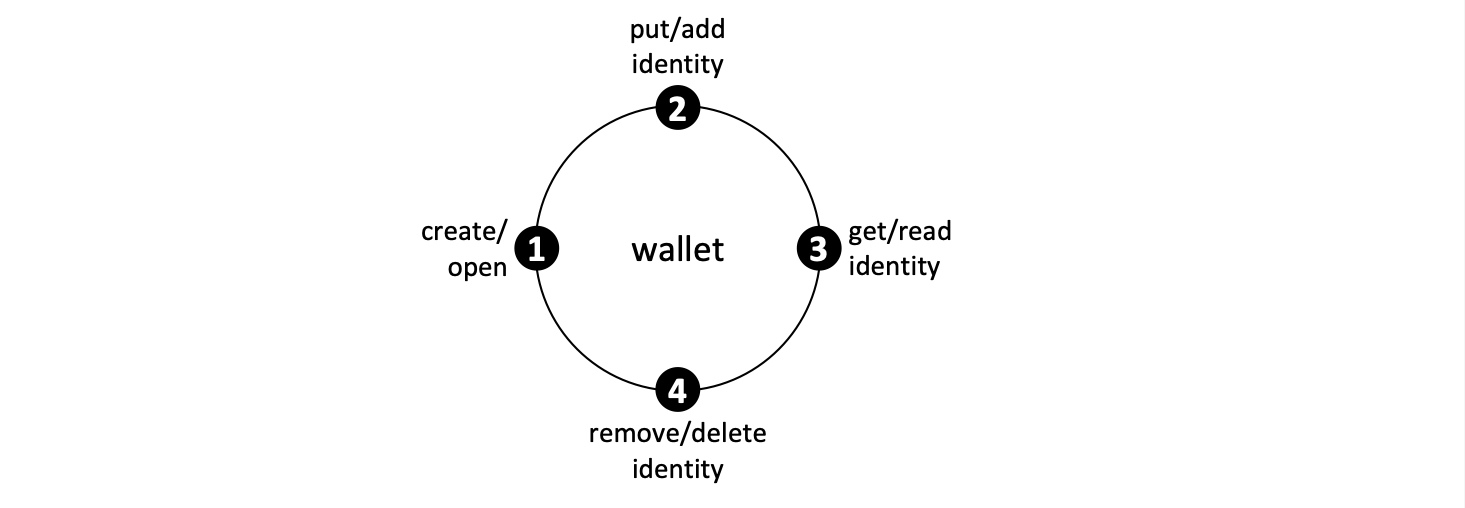
\includegraphics[width=12cm,height=12cm,keepaspectratio]{photos/wallet.png}
    \caption{The architecture and all the operations permissible on the wallet provided by the Hyperledger SDK}
    \label{fig:hyperledger-wallet}
\end{figure}

\bigskip
Once a connection with the channel has been established, we use the NodeJS SDK provided by Hyperledger to invoke the chaincodes on the channel. We have endpoints in our API for different operations and after doing some validations, each endpoint prepares a transaction and passes it along when invoking the chaincode. Once a transaction is submitted the API gets a transaction id and maps it in the cache. And is returned to the caller of the API. Once the transaction is complete the cache is updated. The below listing shows the code when we are creating a block on the chain. The start of the function is cut off for better readability, we create an encryption key and store it against the id of the data, which is the hash of the data to avoid creating duplicates on the chain. The keys are stored in the MySQL database and then we create the data transaction and submit it to the blockchain. And the functions used to encrypt and decrypt the data are also shown in the listing.

\begin{lstlisting}[language=java, caption={Endpoint to create a block in the chain}]
...
const assetId: string = crypto.createHash('sha256').update(JSON.stringify(asset)).digest('hex');
asset.id = assetId;
const volumeDetails = asset.storageType.toLowerCase() == 'azure' ? asset.azure : asset.local;
delete asset.azure;
delete asset.local;
asset.lease = '';
// Encrypt volumeDetails here with a key
const iv = Buffer.from(crypto.randomBytes(16)).toString('hex').slice(0, 16);
const key = crypto.createHash('sha256').update(JSON.stringify(Math.random())).digest('hex').slice(0, 32);
const key_mapping = { id: assetId, crypto_key: key, iv: iv };
const insertedData = await insertData('INSERT INTO key_mappings SET ?', key_mapping);
// Code contracted in this listing
const encryptedVolumeDetails = encrypt(JSON.stringify(volumeDetails), key, iv);
asset.volumeDetails = encryptedVolumeDetails;
try {
const submitQueue = request.app.locals.jobq as Queue;
const jobId = await addSubmitTransactionJob(
  submitQueue,
  mspId,
  'AddDataBlock',
  JSON.stringify(asset)
);
return response.status(202).json({
  status: "Accepted",
  jobId: jobId,
});
}
\end{lstlisting}
\begin{lstlisting}[language=java, caption={Functions used for encrypting and decypting text}]
//Encrypting text
function encrypt(text: string, key: string, iv:string) {
   let cipher = crypto.createCipheriv(ALGORITHM, Buffer.from(key), iv);
   let encrypted = cipher.update(text);
   encrypted = Buffer.concat([encrypted, cipher.final()]);
   return encrypted.toString('hex');
}
// Decrypting text
function decrypt(text: string, key: string, iv:string) {
   let encryptedText = Buffer.from(text, 'hex');
   let decipher = crypto.createDecipheriv('aes-256-cbc', Buffer.from(key), iv);
   let decrypted = decipher.update(encryptedText);
   decrypted = Buffer.concat([decrypted, decipher.final()]);
   return decrypted.toString();
}
\end{lstlisting}

\subsection{JupyterHub}
JupyterHub is used to provide an interface for users from multiple organizations to explore the datasets and use the IDE to write code and workflows. And since it is set up on a Kubernetes cluster the workflows are then triggered on it. It can host multiple single-user Jupyter servers whenever a user logs in. We set up JupyterHub on a local Kubernetes cluster for development and testing. In a production environment, this can be swapped with a multi-node cluster setup where each organization can contribute one or more nodes to the cluster.

\bigskip
As part of the setup we create a Kubernetes service account that will enable JupyterFlow to perform the operations of volume management.
\begin{lstlisting}[caption={Rules for volume-manager service account YAML configuration}]
rules:
- apiGroups: [""]
  resources: ["persistentvolumes"]
  verbs: ["get", "watch", "list", "create", "update", "patch", "delete"]
...
rules:
- apiGroups: [""]
  resources: ["persistentvolumeclaims"]
  verbs: ["get", "watch", "list", "create", "update", "patch", "delete"]
...
rules:
- apiGroups: [""]
  resources: ["secrets"]
  verbs: ["get", "create", "delete"]\end{lstlisting}
The service account can do all the operations on persistent-volume and persistent-volume-claims and only get, create and delete operations on secrets. ClusterRole is a role that can be bound to a service account enabling operations on a cluster level instead of a namespace level. And we create a service account volume manager with the above-created roles bound to it.

\bigskip
We create a docker image with the necessary dependencies like our custom Data Explorer extension and Extended JupyterFlow plugin installed and service account token configured. These are the dependencies necessary for the proof of concept to function. The token for the service account is configured as an environment variable. To start up the JupyterHub Instance on the cluster, we have a script \lstinline{runJupyterhub.sh}. When run, it adds JupyterHub helm repositories and Argo helm repositories and applies them to start JupyterHub and Argo deployments on Kubernetes, using a \lstinline{config.yaml} file specifying the docker image for spawning Jupyter instances and some configurations for that. A complete list of details can be found at \footnote{\url{https://zero-to-jupyterhub.readthedocs.io/en/latest/jupyterhub/customizing/user-environment.html}}. Helm is a package management tool for Kubernetes deployments. The Argo helm repo also creates a service exposing the servers to the host machine. And finally, we create a headless service in Kubernetes for allowing the cluster to call the REST API hosted on another machine.

\begin{lstlisting}[caption={Configuration for a headless service on Kubernetes}]
apiVersion: v1
kind: Service
metadata:
   name: blockchain-service
spec:
   clusterIP: None
   ports:
   - protocol: TCP
     port: 3000
     targetPort: 3000
   type: ClusterIP
---
apiVersion: v1
kind: Endpoints
metadata:
  name: blockchain-service
subsets:
  - addresses:
      - ip: 
    ports:
      - port: 3000
\end{lstlisting}

\subsection{Extension}
The extension is a React JupyterLab extension enabling end-users to view the datasets available, submit transactions to consume them in workflows, and admin users to do administrative tasks. \ref{fig:extension} Shows how the extension looks like. We emphasize again that the Wallet id and is admin are simple input fields which will be removed upon integration with Distributed Identity framework and the respective values received from DID framework.

\begin{figure}
    \centering
    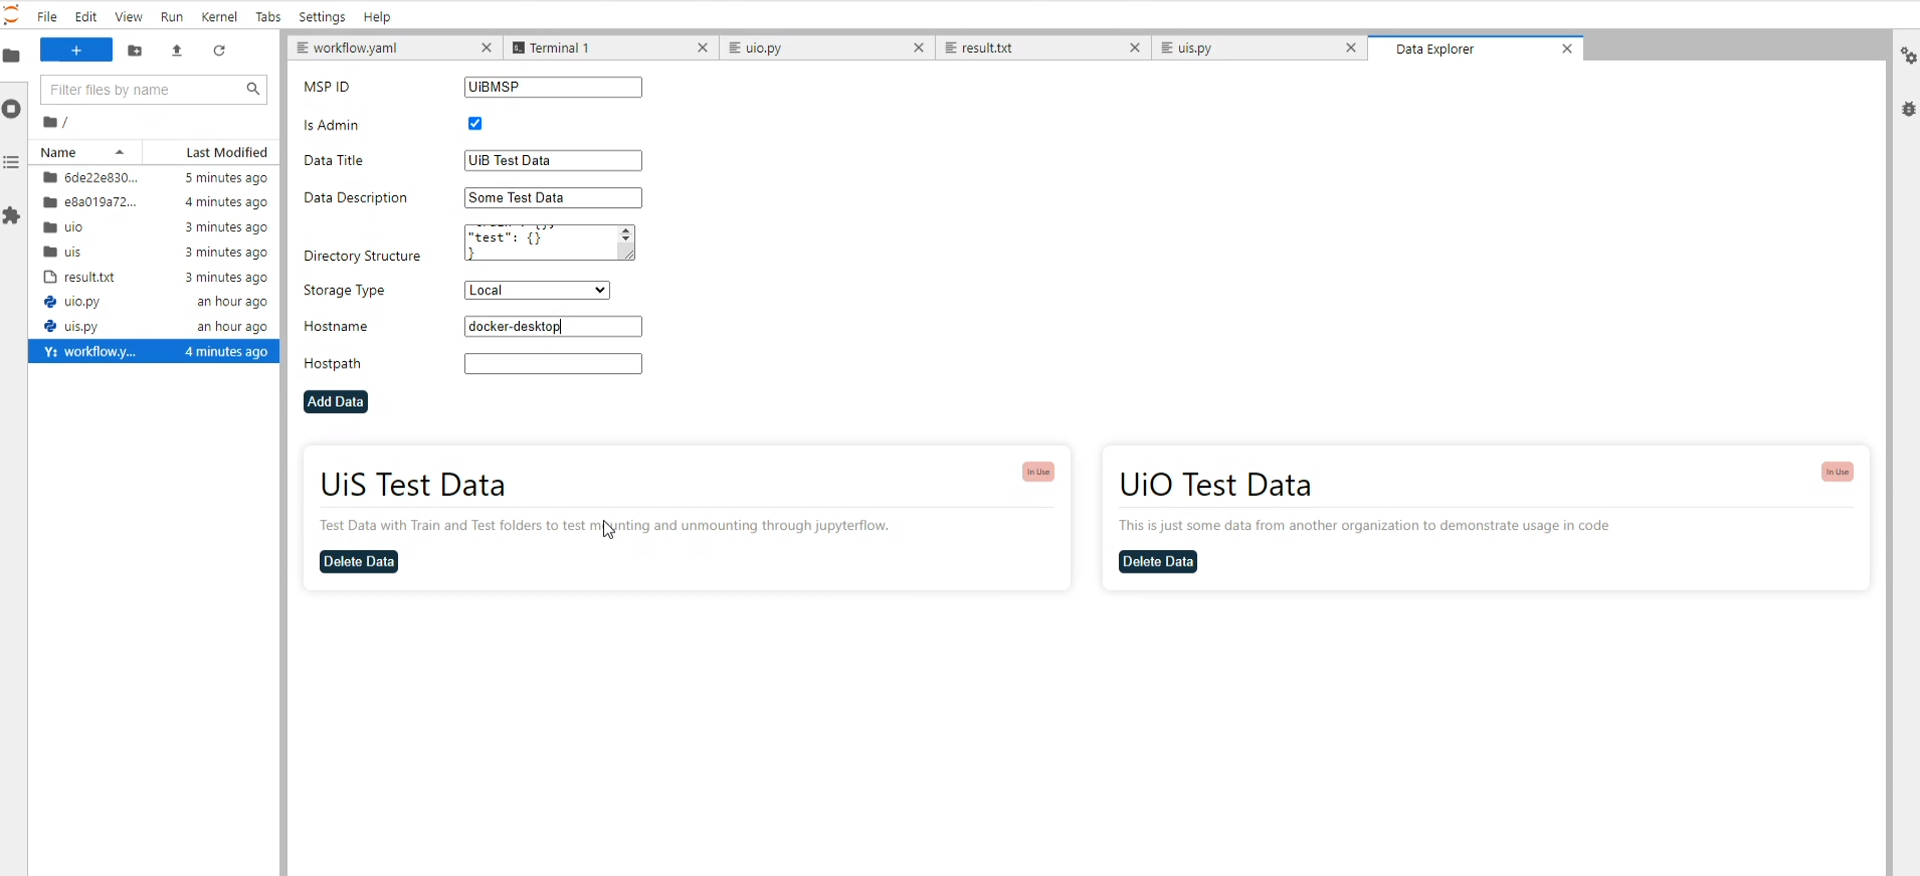
\includegraphics[width=14cm,keepaspectratio]{photos/Extension Screenshot.png}
    \caption{Screenshot of the extension in the proof of concept.}
    \label{fig:extension}
\end{figure}

\bigskip
Upon selection of a dataset for consumption, the extension creates a directory structure of the dataset in question with an id as the root of this directory structure. The user can write code experimenting with that directory structure. The extension also gets the decrypted sensitive information that can be used to mount the dataset and sets them in a hidden file on the File System. As mentioned before right now it is only secured by obscuring the information and hiding it from the user and can be improved upon in later work.

\subsection{JupyterFlow}
The last piece of the puzzle is JupyterFlow. It enables the users to run complex, compute-intensive workflows on a Kubernetes cluster while removing all the complexities of writing complicated YAML files for Argo and containerizing the code and the environment. 

\bigskip
We have extended the JupyterFlow to enable users to specify the volumes that a job in the workflow consumes and mount that volume before triggering the workflow. \ref{lst:basic-jflow} shows the basic YAML files that users could write to design complex workflows and JupyterFlow will convert it to the respective Argo Workflow and trigger it. \ref{lst:new-jflow} Is the YAML in our extended JupyterFlow plugin. The users can now specify the volumes as part of the jobs and these volumes will be mounted and consumed by that job only once the workflow is triggered. The id is received from the extension when a dataset is selected, the name can be a random name and the path is the path to mount the volume inside the container. 'dags' is the section describing workflow dependencies and the order to run the jobs in. The index starts at 1 for the first job, so the following workflow will run job 1 then after it has succeeded will run job 2 and job 3 in parallel.

\begin{lstlisting}[caption={YAML for mounting volumes using JupyterFlow in workflows in our custom JupyterFlow},label={lst:new-jflow}]
jobs:
- command: 'pwd' 
- command: 'ls -la /home/jovyan/uis'
  volumes:
  - id: ''
    name: ''
    path: ''
- command: 'ls'

dags:
- 1 >> 2
- 1 >> 3
\end{lstlisting}